\chapter{Architektura systemu}
Architektura budowanego systemu nie będzie skomplikowana. Całość uruchamiana
będzie na jednej maszynie -- serwerze. Całość, to znaczy: aplikacja internetowa, scheduler
oraz Dispatch Rider.
\section{Aplikacja internetowa}
Aplikacja internetowa to miejsce, w którym użytkownik będzie mógł łączyć się z systemem.
Zostanie napisana między innymi przy użyciu języka PHP, co oznacza, że na serwerze,
na którym zostanie uruchomiona aplikacja konieczna będzie jego obsługa.

Najważniejsze z punktu widzenia całego systemu będą znajdujące się w niej 2 katalogi: \texttt{uploads}
oraz \texttt{ready}. W pierwszym będą pojawiać się pliki z właściwościami i konfiguracją wysyłane przez 
użytkownika. Każdy zestaw plików w osobnym folderze o nazwie utworzonej z nazwy wybranej przy uploadzie
przez użytkownika. Pliki te będzie można edytować z poziomu aplikacji www do momentu, aż nie zostaną
przejęte przez schedulera do dalszego przetwarzania. Po zakończeniu przetwarzania problemu przez Dispatch
Ridera, pliki wynikowe wylądują w folderze \texttt{ready}. Aplikacja internetowa będzie przeglądać
każdy z tych katalogów w celu wyświetlenia użytkownikowi informacji na temat przebiegu przetwarzania.

Poza tym w aplikacji internetowej będzie można podejrzeć graf problemu zbudowany w oparciu o pliki
wynikowe z Dispatch Ridera, co jest głównym celem tego projektu. Graf będzie utworzony przy pomocy
biblioteki \texttt{JavaScript InfoVis Toolkit}.

\section{Scheduler}
Scheduler to osobna aplikacji napisana w Javie służąca do kolejkowania zadań przesłanych do systemu
przez użytkownika. Skanuje ona zawartość folderów \texttt{uploads} i \texttt{ready} z aplikacji internetowej
i zarządza ich przesyłaniem do Dispatch Ridera. Scheduler jest więc łącznikiem pomiędzy usługą kliencką,
a serwerową. W momencie ukończenia przetwarzania problemu przez Dispatch Ridera scheduler przenosi pliki
wynikowe do odpowiedniego podfolderu katalogu \texttt{ready} i w sytuacji gdy jakiś problem czeka już w kolejce
do obliczeń, przesyła go do Dispatch Ridera.

\section{Dispatch Rider}
Serce całego systemu. Aplikacja, która zajmuje się wykonywaniem wszystkich obliczeń związanych z danym problemem.
Wykorzystana będzie gotowa już aplikacja, napisana przez naszych starszych kolegów, w którą nię będziemy
ingerować, a jedynie skorzystamy z jej plików wynikowych. Aplikacja jest uruchamiana i zarządzana przez schedulera.

\section{Diagram komponentów systemu}

\begin{center}
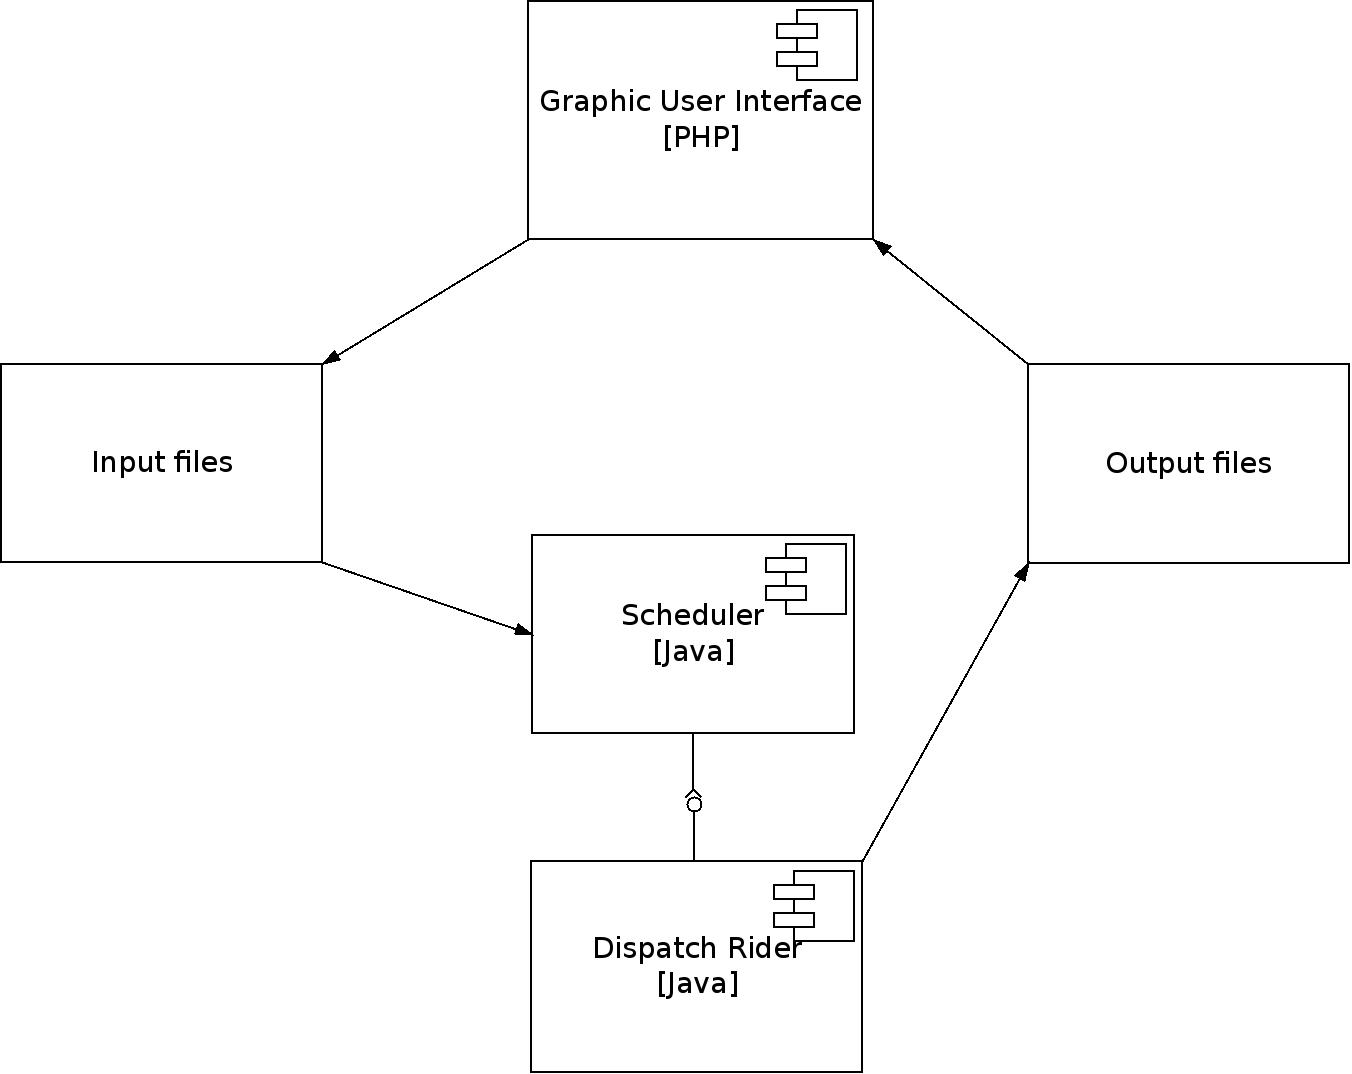
\includegraphics[scale=0.35]{imgs/IO.jpeg}
\end{center}